\begin{recipe}{叉烧宣腿}

\ingredients

\ingredient{宣腿}{二斤}
\ingredient{荷叶饼}{十二个}
\ingredient{面包}{八两}
\ingredient{干豆粉}{三钱}
\ingredient{鸡蛋}{二个}

\preparation

\step 选用硬边宣腿一方,用温水洗净,用刀将附于火腿上的黑色薄皮刮尽。

\begin{wrapfigure}[13]{l}{11em}%
\centering%
\vspace{-.75\baselineskip}%
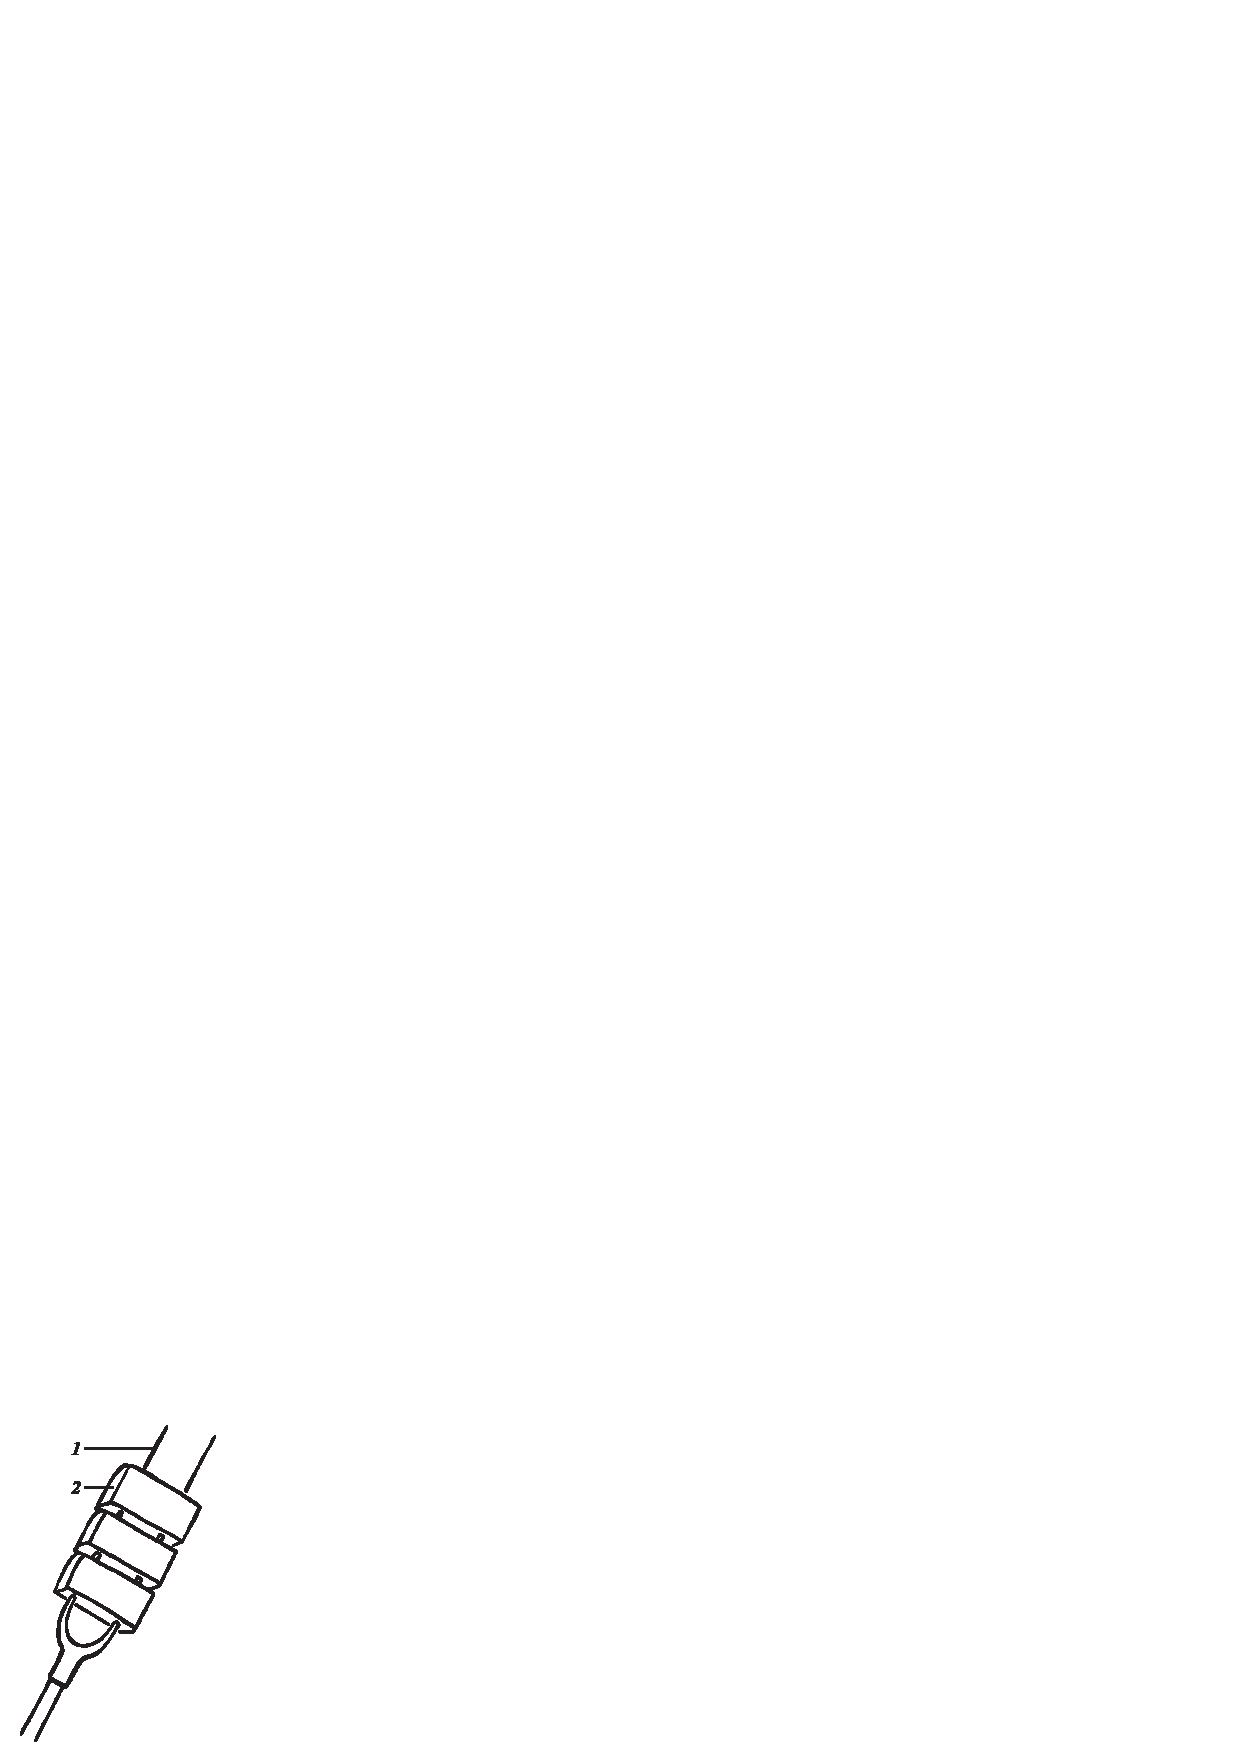
\includegraphics[scale=1]{illustration-011.pdf}%
\vspace{-.4375\baselineskip}%
\caption{叉烧宣腿叉法}
\label{叉烧宣腿}%
\begingroup%
\small%
\noindent%
\null\hspace{0em}1. 铁叉 2. 火腿
\endgroup%
\end{wrapfigure}

\step 用刀将火腿均匀地切为三块,每块切成一寸三分宽、四寸半长,厚度为火腿本身的
厚度,用铁叉平叉起来(如图\,\ref{叉烧宣腿}\,)。将蛋清与豆粉调匀,涂于叉起来的
火腿上以保持原味,而免烧时走油走味。

\step 把杠炭三斤放入平炉上烧红,而后把叉好的火腿在平炉上以微火烘烤,要反复转动
叉柄,约二十分钟,烤至火腿熟透心时,揩净叉尖后取下叉子。用刀把火腿每隔两分远切
一刀,但不要完全切断,使其不会分开。然后摆在盘中,下面摆两块、上面摆一块成为
“品”字形。与烤熟的面包(切为十二片)和蒸好的荷叶饼同时上席。

\features

此菜外酥内香,为下酒的好菜。

\end{recipe}

% vim: filetype=tex noautoindent nojoinspaces
% vim: fileencoding=utf-8 formatoptions+=m
% vim: textwidth=78 tabstop=4 shiftwidth=4 softtabstop=4
